\documentclass{article}
\usepackage{graphicx}
\usepackage{float}
\usepackage{hyperref}
\usepackage{caption}
\begin{document}
	\title{\textbf{Heart Disease Data Report}}
	\author{Snehal Suhane \\ 12342100} 
	
	\date{}
	\maketitle
	
	\section*{Heart Disease Dataset}
	
	
	\section{Gender vs Number of People with Heart Disease}
	Figure \ref{fig:fig1} shows the distribution of heart disease across genders. The x-axis represents gender (0 = Female, 1 = Male), while the y-axis shows the number of people with heart disease in each gender group. This helps to visualize any potential correlation between gender and the incidence of heart disease.
	\begin{figure}[h]
		\centering
		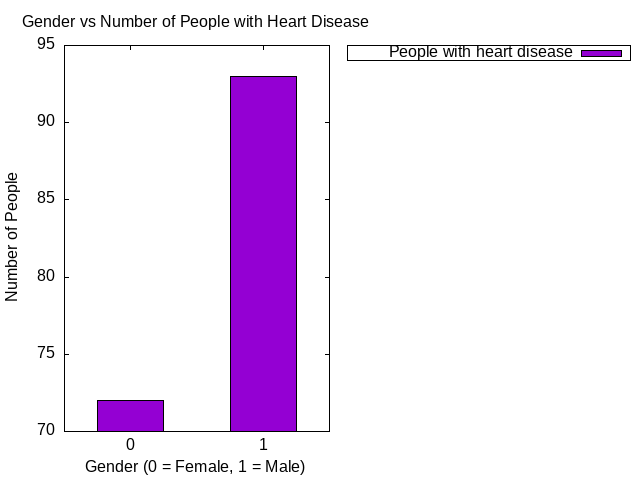
\includegraphics[width=0.8\textwidth]{../que4a/que4a.png}
		\caption{Gender vs Number of People with Heart Disease}
		\label{fig:fig1}
	\end{figure}
	\section{Age vs Blood Pressure}
	Figure \ref{fig:fig2} illustrates the relationship between age (x-axis) and blood pressure (y-axis). Each point represents an individual data entry from the dataset. This plot is useful for identifying any trend or correlation between age and blood pressure, which could be relevant in analyzing risk factors for heart disease.
	\begin{figure}[h]
		\centering
		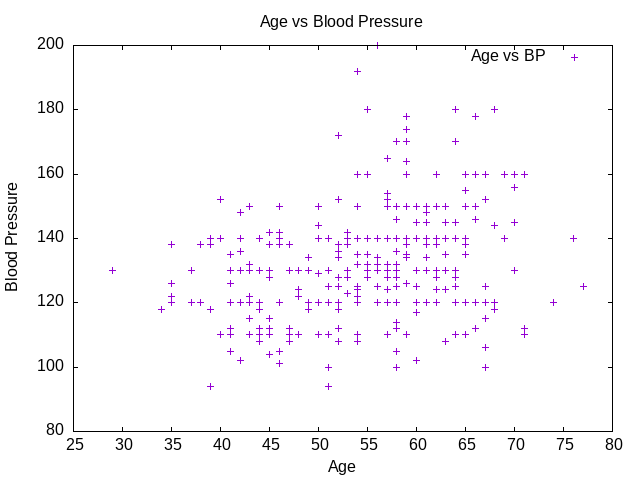
\includegraphics[width=0.8\textwidth]{../que4b/que4b.png}
		\caption{Age vs Blood Pressure}
		\label{fig:fig2}
	\end{figure}
	\section{Age vs Cholesterol (No Heart Disease)}
	Figure \ref{fig:fig3} represents the correlation between age and cholesterol levels specifically for individuals who do not have heart disease. The x-axis denotes age, while the y-axis represents cholesterol levels. By focusing only on non-heart disease cases, we can observe if there are age-related trends in cholesterol independent of heart disease.
	\begin{figure}[h]
		\centering
		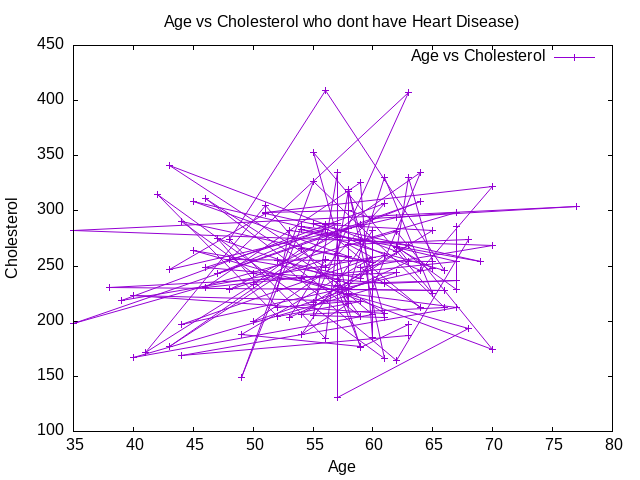
\includegraphics[width=0.8\textwidth]{../que4c/que4c.png}
		\caption{Age vs Cholesterol (No Heart Disease)}
		\label{fig:fig3}
	\end{figure}
	\section{Percentage of Age Groups with Heart Disease}
	Figure \ref{fig:fig4} shows the distribution of heart disease cases across different age groups (40-50, 50-60, etc.). Each segment represents the percentage of individuals with heart disease in a specific age range. This visualization helps to highlight age groups where heart disease is more prevalent, assisting in targeted analysis of age as a factor in heart disease risk
	\begin{figure}[h]
		\centering
		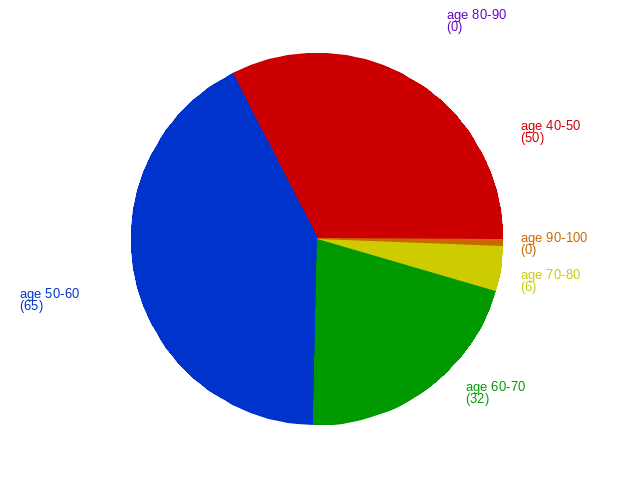
\includegraphics[width=0.8\textwidth]{../que4d/que4d.png}
		\caption{Percentage of Age Groups with Heart Disease}
		\label{fig:fig4}
	\end{figure}
	
\end{document}